\section{Extension}
Nous avons décidé d'implémenter l'extension 2 en introduisant des agents menteurs. Ces mensonges interviennent dans les deux composantes suivantes : WR et CR. Les consommateurs peuvent fournir de fausses notes lorsque le fournisseur leur demande une certification ou quand un autre consommateur les contacte pour un témoignage. Pour ce dernier, nous avions pensé à deux alternatives : inventer une interaction qui n'a jamais eu lieu et envoyer la fausse note ou se baser sur l'ensemble de notes existant pour le modifier. Cette dernière a été choisie car elle permet de garder une certaine logique dans les fausses notes : qu'ils proviennent de CR ou WR, il s'agit toujours d'un écart par rapport à une vraie note. Ce genre de notes biaisées nous semblait être le plus réaliste et le plus commun.
Nous avons posé un intervalle [-0.75,0.75] dans lequel une valeur $\epsilon$ sera tirée aléatoirement. Ainsi \[NewRate = OldRate + \epsilon\].
\subsection{Résutats}
Contrairement à nos attentes, les agents s'en sortent plutôt bien. Ce qui montre que le modèle FIRE est robuste aux mensonges.

\begin{figure}[H]
    \begin{minipage}{0.3\textwidth}
     \centering
     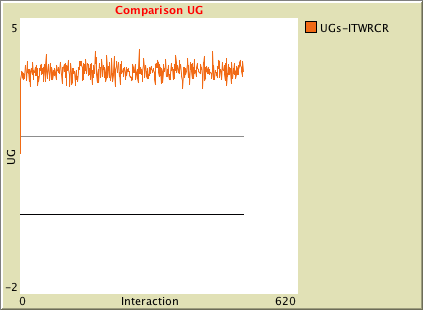
\includegraphics[width=.6\linewidth]{images/evolutionLiars/20.png}
     \caption{20\% de menteurs}\label{Fig:Data2}
   \end{minipage}
   \begin{minipage}{0.3\textwidth}
     \centering
     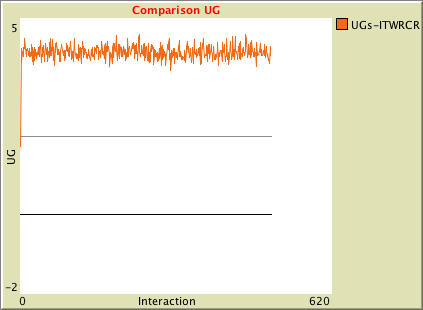
\includegraphics[width=.6\linewidth]{images/evolutionLiars/50.png}
     \caption{50\% de menteurs}\label{Fig:Data1}
   \end{minipage}
   \begin{minipage}{0.3\textwidth}
     \centering
     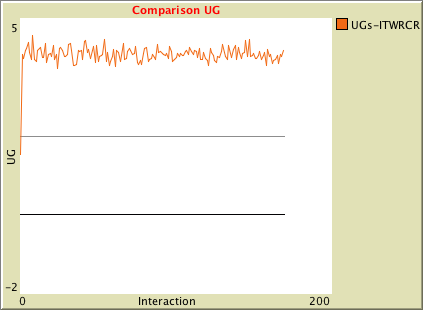
\includegraphics[width=.6\linewidth]{images/evolutionLiars/80.png}
     \caption{80\% de menteurs}\label{Fig:Data2}
   \end{minipage}
\end{figure}



